\section{What is a pointer?}
\begin{itemize}
    \item A variable.
        \begin{itemize}
            \item Whose value is an address.
        \end{itemize}

    \item What can be at that address?
        \begin{itemize}
            \item Another variable.
            \item A function.
        \end{itemize}
    
    \item Pointers have a memory location that is bound to, type and has a value, this value is address in memory.
    \item If x is an integer variable and its value is 10 then I can declare a pointer that points to it.
    \item To use the data that the pointer is pointing to you must know its type.
\end{itemize}

\subsection{Why use pointers?}
\begin{itemize}
    \item Can't I just use the variable or the function itself?
        \begin{itemize}
            \item Yes, but you can't always do that.
        \end{itemize}
    
    \item Inside functions, pointers can be used to access data that are defined outside the function. Those values may not be in scope so you can't access them by their name.
    \item Pointers can be used to operate on arrays very efficiently.
    \item We can allocate memory dynamically on the heap or free store.
        \begin{itemize}
            \item This memory doesn't even have a variable name.
            \item The only way to get to it is via a pointer.
        \end{itemize}
    
    \item With object-oriented programming,  pointers are how polymorphism works.
    \item Can access specific addresses in memory.
        \begin{itemize}
            \item Useful in embedded and system applications.
        \end{itemize}
\end{itemize}


%----------------------------------------------------------------------------------------
\section{Declaring pointer variables}
\begin{itemize}
    \item We declare pointer variables in very much the same way any other variable would, except an asterisk must be between the type and the identifier:
        \begin{verbatim}
            variable_type *pointer_name;
        \end{verbatim}
        \begin{minted}[autogobble]{cpp}
            int *int_ptr; // pointer to int.
            double *double_ptr; // pointer to double.
            char *char_ptr; // pointer char.
            std::string *string_ptr; // pointer to a std::string.
        \end{minted}
        \begin{itemize}
            \item Keep in mind that there are many conventions to declaration of pointers, such as the one where the asterisk is next to the type \mintinline{cpp}{int* name;}, others where the asterisk is previous to the name \mintinline{cpp}{int *name;} or even a space from each \mintinline{cpp}{int * name;}
        \end{itemize}
    
    \item Intializing pointer variables to ``point no where'' or null:
        \begin{itemize}
            \item If you don't initialize your pointers they will have garbage data.
            \item In this case that data will be addresses.
            \item Just as an int was as convention initialized to a value, say 0, a pointer is usually initialized to null which means it doesn't point to any memory location. 
            \item You do this with the \mintinline{cpp}{nullptr} or the \mintinline{cpp}{NULL} keywords.
        \end{itemize}
        \begin{verbatim}
            variable_type *pointer_name {nullptr};
        \end{verbatim}
        \begin{minted}[autogobble]{cpp}
            int *int_ptr {};
            double *double_ptr {nullptr};
            char *char_ptr {nullptr};
            string *string_ptr {nullptr};
        \end{minted}
    
    \item Always initialize variable pointers to 'point no where 'or null.
        \begin{itemize}
            \item Always initialize.
            \item Uninitialized pointers contain garbage data and can 'point anywhere' in memory.
            \item Initializing to zero or \mintinline{cpp}{nullptr} (C++11) represents address zero.
                \begin{itemize}
                    \item Implies that the pointer is 'pointing nowhere'.
                \end{itemize}
            
            \item If you don't initialize a pointer to point to a variable or function then you should initialize it to \mintinline{cpp}{nullptr} to 'make it null'.
        \end{itemize}
\end{itemize}


%----------------------------------------------------------------------------------------
\section{Accessing the pointer address and storing address in a pointer}
\begin{itemize}
    \item The address operator.
        \begin{itemize}
            \item Variables are stored in unique addresses.
            \item Unary operator.
            \item Evaluates to the address of its operand.
                \begin{itemize}
                    \item Operand cannot be a constant or expression that evaluates to temp values.
                \end{itemize}
        \end{itemize}
        \begin{minted}[autogobble]{cpp}
            #include <iostream>
            using namespace std;
            int main() {
                int num{10};
                cout << "Value of num is: " << num << endl;
                cout << "Size of num is: " << sizeof num << endl;
                cout << "Address of num is: " << &num << endl;
                return 0;
            }
            /* OUTPUT:
            Value of num is: 10
            Size of num is: 4
            Address of num is: 0x61fe1c
            */
        \end{minted}
    
    \item Example:
        \begin{minted}[autogobble]{cpp}
            #include <iostream>
            using namespace std;
            int main() {
                int *p;
                cout << "Value of p is: " << p << endl; // garbage data.
                cout << "Address of p is: " << &p << endl; // value of p.
                cout << "Size of p is: " << sizeof p << endl; // size of p.
                p = nullptr;
                cout << "Value of p is: " << p << endl;
                return 0;
            }
            /* OUTPUT:
            Value of p is: 0x10
            Address of p is: 0x61fe18
            Size of p is: 8
            Value of p is: 0

            */
        \end{minted}
\end{itemize}

\subsection{sizeof a pointer variable}
\begin{itemize}
    \item Don't confuse the size of a pointer variable and the size of what it points to.
    \item All pointers in a program have the same size.
    \item They may be pointing to a very large or very small types.
\end{itemize}
\begin{minted}[autogobble]{cpp}
    int *p1 {nullptr};
    double *p2 {nullptr};
    unsigned long long *p3 {nullptr};
    vector<string> *p4 {nullptr};
    string *p5 {nullptr};
\end{minted}

\subsection{Storing an address in a pointer variable?}
Typed pointers.
\begin{itemize}
    \item The compiler will make sure that the address stored in a pointer variable is of the correct type.
\end{itemize}
\begin{minted}[autogobble]{cpp}
    int score {10};
    double high_temp {100.7};
    int *score_ptr {nullptr};
    score_ptr = &score;
    score_ptr = &high_temp; // compiler error because high_temp is a double and score_ptr is an int.
\end{minted}

\subsection{\& the address of operator}
\begin{itemize}
    \item Pointers are variables so they can change.
    \item Pointers can be null.
    \item Pointers can be uninitialized.
\end{itemize}



%----------------------------------------------------------------------------------------
\section{Dereferencing the pointer}
\begin{itemize}
    \item Access the data we're pointing to is called dereferencing a pointer.
    \item If \verb|score_ptr| is a pointer and has a valid address.
    \item Then you can access the data at the address contained in the \verb|score_ptr| using the dereferencing operator.
        \begin{minted}[autogobble]{cpp}
            #include <iostream>
            using namespace std;
            int main() {
                int score {100};
                int *score_ptr {&score};
                cout << *score_ptr << endl; // 100
                *score_ptr = 200;
                cout << *score_ptr << endl;
                cout << score << endl;
                return 0;
            }
            /* OUTPUT:
            100
            200
            200
            */
        \end{minted}
        \begin{itemize}
            \item Declaring and dereferencing is done using the asterisk, C++ has received some criticism about this, but once you understand where and how to use the asterisk you'll be fine.
        \end{itemize}

    
    \item Example:
        \begin{minted}[autogobble]{cpp}
            #include <iostream>
            #include <vector>
            using namespace std;
            int main() {
                vector<string> stooges {"Larry", "Moe", "Curly"};
                vector<string> *vector_ptr {nullptr};
                vector_ptr = &stooges;
                cout << "First stooge: " << (*vector_ptr).at(0) << endl;
                cout << "Stooges: ";
                for (auto stooge: *vector_ptr) {
                    cout << stooge << " ";
                }
                cout << endl;
                return 0;
            }
            /* OUTPUT:
            First stooge: Larry
            Stooges: Larry Moe Curly
            */
        \end{minted}
\end{itemize}


%----------------------------------------------------------------------------------------
\section{Dynamic Memory Allocation}
\begin{itemize}
    \item Allocating storage from the heap at runtime.
    \item We often don't knot how much storage we need until we need it.
    \item We can allocate storage for a variable at run time.
    \item Recall C++ arrays:
        \begin{itemize}
            \item We had to explicitly provide the size and it was fixed.
            \item But vectors grow and shrink dynamically.
        \end{itemize}
    
    \item We can use pointers to access newly allocated heap storage.
\end{itemize}

\subsection{Allocating and deallocating memory}
\begin{itemize}
    \item The \mintinline{cpp}{new} keyword
        \begin{itemize}
            \item Using the new keyword to allocate storage.
            \begin{minted}[autogobble]{cpp}
                #include <iostream>
                using namespace std;
                int main() {
                    int *int_ptr {nullptr};
                    int_ptr = new int; // allocate an integer on the heap.
                    cout << int_ptr << endl; // address of int_ptr.
                    cout << *int_ptr << endl; // garbage. Notice the dereferencing.
                    *int_ptr = 100;
                    cout << *int_ptr << endl; // 100.
                    return 0;
                }
                /* OUTPUT:
                0x25824f0
                39331936
                100
                */
            \end{minted}
    
        \item If you loose the pointer because it goes out of scope or other such incidents, that is called a memory leak and you lost the only way you have to access that memory.
        \item You also must deallocate the pointer after you are done using it.
        \end{itemize}
    
    \item The \mintinline{cpp}{delete} keyword
        \begin{itemize}
            \item The delete keyword is used to deallocate allocated space.
                \begin{minted}[autogobble]{cpp}
                    int *int_ptr {nullptr}; // allocate an integer on the heap.
                    delete int_ptr; // frees the allocated storage.
                \end{minted}
        \end{itemize}
    
    \item The \mintinline{cpp}{new[]} keyword
        \begin{itemize}
            \item The \mintinline{cpp}{new[]} is used to allocate an array.
                \begin{minted}[autogobble]{cpp}
                    int *array_ptr {nullptr};
                    int size {};
                    cout << "How big do you want the array: ";
                    cin >> size;
                    array_ptr = new int[size]; // allocate array on the heap.
                \end{minted}
            \item Keep in mind that these brackets must be empty.
        \end{itemize}
    

    \item The \mintinline{cpp}{delete[]} keyword is used to deallocate storage of an array.
        \begin{minted}[autogobble]{cpp}
            int *array_ptr {nullptr};
            int size {};
            cout << "How big do you want the array: ";
            cin >> size;
            array_ptr = new int[size]; // allocate array on the heap.
            delete[] array_ptr; // free allocated storage.
        \end{minted}
        \begin{itemize}
            \item Keep in mind that these brackets must be empty.
        \end{itemize}
    
    \item When you allocate dynamically you are allocating into the heap or the free store, the stack houses the pointer to the dynamically allocated data.
        \begin{itemize}
            \item Example:
                \begin{minted}[autogobble]{cpp}
                    #include <iostream>
                    using namespace std;
                    int main() {
                        size_t size{0}; // allocated on the stack.
                        double *temp_ptr {nullptr}; // allocated on the stack.
                        cout << "How many temps: "; 
                        cin >> size;
                        temp_ptr = new double[size]; // allocated on the heap.
                        cout << temp_ptr << endl;
                        delete[] temp_ptr; // dealocated on the heap.
                        return 0;
                    }
                \end{minted}
        \end{itemize}
\end{itemize}



%----------------------------------------------------------------------------------------
\section{Relationship between arrays and pointers}
\begin{itemize}
    \item The value of an array name is the address of the first element in the array.
    \item The value of a pointer variable is an address.
    \item If the pointer points to the same data types as the array element then the pointer and array name can be used interchangeably (almost).
        \begin{minted}[autogobble]{cpp}
            #include <iostream>
            using namespace std;
            int main() {
                int scores[] {100,95,89};
                cout << scores << endl;
                cout << *scores << endl;
                int *score_ptr {scores};
                cout << score_ptr << endl;
                cout << *score_ptr << endl;
                return 0;
            }
            /* OUTPUT:
            0x61fe0c
            100
            0x61fe0c
            100
            */
        \end{minted}
    
    \item We can also use array subscripting on a pointer using the square brackets operator.
        \begin{minted}[autogobble]{cpp}
            #include <iostream>
            using namespace std;
            int main() {
                int scores[] {100,95,89};
                int *score_ptr {scores};
                cout << score_ptr[0] << endl;
                cout << score_ptr[1] << endl;
                cout << score_ptr[2] << endl;
                return 0;
            }
            /* OUTPUT:
            100
            95
            89
            */
        \end{minted}
    
    \item You can perform pointer arithmetic, which is adding numbers to a pointer:
        \begin{minted}[autogobble]{cpp}
            #include <iostream>
            using namespace std;
            int main() {
                int scores[] {100,95,89};
                int *score_ptr {scores};
                cout << score_ptr << endl;
                cout << (score_ptr + 1) << endl;
                cout << (score_ptr + 2) << endl;
                return 0;
            }
            /* OUTPUT:
            0x61fe0c
            0x61fe10
            0x61fe14
            */
        \end{minted}
        \begin{minted}[autogobble]{cpp}
            #include <iostream>
            using namespace std;
            int main() {
                int scores[] {100,95,89};
                int *score_ptr {scores};
                cout << *score_ptr << endl;
                cout << *(score_ptr + 1) << endl;
                cout << *(score_ptr + 2) << endl;
                return 0;
            }
            /* OUTPUT:
            100
            95
            89
            */
        \end{minted}
\end{itemize}

\subsection{Subscript and offset notation equivalence}
\begin{itemize}
    \item You can write this in two ways:
        \begin{minted}[autogobble]{cpp}
            int array_name[] {1,2,3,4,5};
            int *pointer_name {array_name};
        \end{minted}
    
    \item Subscript notation:
        \begin{minted}[autogobble]{cpp}
            array_name[index];
            pointer_name[index];
        \end{minted}
    
    \item Offset notation:
        \begin{minted}[autogobble]{cpp}
            *(array_name + index);
            *(pointer_name + index);
        \end{minted}
\end{itemize}


%----------------------------------------------------------------------------------------
\section{Pointer arithmetic}
\begin{itemize}
    \item Pointers can be used in:
        \begin{itemize}
            \item Assignment expressions.
            \item Arithmetic expressions.
            \item Comparison expressions.
        \end{itemize}
    
    \item C++ allows pointer arithmetic.
    \item Pointer arithmetic only makes sense with raw arrays.
\end{itemize}

\subsection{++ and --}
\begin{itemize}
    \item ++ increments a pointer to point to the next array element.
        \begin{minted}[autogobble]{cpp}
            int_ptr++;
        \end{minted}
    \item -- decrements a pointer to point to the previous array element.
        \begin{minted}[autogobble]{cpp}
            int_ptr--;
        \end{minted}
    
    \item Keep in mind that in pointer arithmetic, adding one means adding whatever number of bytes the elements occupy in order to get to the next element.
\end{itemize}

\subsection{+ and -}
\begin{itemize}
    \item + increment pointer by some number: (\mintinline{cpp}{n * sizeof(type)})
        \begin{minted}[autogobble]{cpp}
            int_ptr += n; or int_ptr = int_ptr + n;
        \end{minted}
    
    \item - decrement pointer by some number: (\mintinline{cpp}{n * sizeof(type)})
        \begin{minted}[autogobble]{cpp}
            int_ptr -= n; or int_ptr = int_ptr - n;
        \end{minted}
\end{itemize}

\subsection{Subtracting two pointers}
\begin{itemize}
    \item Determine the number of elements between the pointers.
    \item both pointers must point to the same data type:
        \begin{minted}[autogobble]{cpp}
            int n = int_ptr2 - int_ptr1;
        \end{minted}
\end{itemize}

\subsection{Compare two pointers == and !=}
\begin{itemize}
    \item Determine if two pointers point to the same location.
        \begin{itemize}
            \item Does not compare the data where they point.
        \end{itemize}
        \begin{minted}[autogobble]{cpp}
            #include <iostream>
            using namespace std;
            int main() {
                string s1 {"Frank"};
                string s2 {"Frank"};
                string *p1 {&s1};
                string *p2 {&s2};
                string *p3 {&s1};
                cout << boolalpha;
                cout << (p1 == p2) << endl; 
                cout << (p1 == p3) << endl; 
                return 0;
            }
            /* OUTPUT:
            false
            true
            */
        \end{minted}
\end{itemize}

\subsection{Comparing the data pointers point to}
\begin{itemize}
    \item Determine if two pointers point to the same data.
    \item You must compare the referenced pointers.
        \begin{minted}[autogobble]{cpp}
            #include <iostream>
            using namespace std;
            int main() {
                string s1 {"Frank"};
                string s2 {"Frank"};
                string *p1 {&s1};
                string *p2 {&s2};
                string *p3 {&s1};
                cout << boolalpha;
                cout << (*p1 == *p2) << endl; 
                cout << (*p1 == *p3) << endl; 
                return 0;
            }
            /* OUTPUT:
            false
            true
            */
        \end{minted}
\end{itemize}

\subsection{Examples}
\begin{minted}[autogobble]{cpp}
    #include <iostream>
    using namespace std;
    int main() {
        int scores[] {100,95,89,68,-1};
        int *score_ptr {scores};
        while (*score_ptr != -1) {
            cout << *score_ptr << endl;
            score_ptr++;
        }
        return 0;
    }
    /* OUTPUT:
    100
    95
    89
    68
    */
\end{minted}

\begin{minted}[autogobble]{cpp}
    #include <iostream>
    using namespace std;
    int main() {
        char name[] {"Frank"};
        char *char_ptr1 = &name[0];
        char *char_ptr2 = &name[3];
        cout << "In the string " << name << ", " << *char_ptr2 << " is " << (char_ptr2 - char_ptr1) << " characters away from " << *char_ptr1 << endl;
        return 0;
    }
    /* OUTPUT:
    In the string Frank, n is 3 characters away from F
    */
\end{minted}


%----------------------------------------------------------------------------------------
\section{Passing pointers to a function}
const and pointers:
\begin{itemize}
    \item There are several ways to qualify pointers using const.
        \begin{itemize}
            \item Pointers to constants.
            \item Constant pointers.
            \item Constant pointers to constants.
        \end{itemize}
    
    \item Pointers to constants:
        \begin{itemize}
            \item The data pointed to by the pointers is constant and cannot be changed.
            \item The pointer itself can change and point somewhere else.
            \item Pointers to constants follow the syntax: \verb|const type *var_name|.
        \end{itemize}
        \begin{minted}[autogobble]{cpp}
            int high_score {100};
            int low_score {65};
            const int *score_ptr {&high_score};
            *score_ptr = 86; // error, changing the data being pointed to.
            score_ptr = &low_score; // Ok.
        \end{minted}
    
    \item Constant pointers:
        \begin{itemize}
            \item The data pointed to by the pointers can be changed.
            \item The pointer itself cannot change and point somewhere else.
            \item Const pointers follow the syntax: \verb|type const *var_name|.
        \end{itemize}
        \begin{minted}[autogobble]{cpp}
            int high_score {100};
            int low_score {65};
            int const *score_ptr {&high_score};
            *score_ptr = 86; // Ok.
            score_ptr = &low_score; // Error, changing the pointer.
        \end{minted}
\end{itemize}


%----------------------------------------------------------------------------------------
\section{Passing pointers to functions}
\begin{itemize}
    \item Pass-by-reference with pointer parameters.
    \item We can use pointers and the dereference operator to achieve pass-by-reference.
    \item The function parameter is a pointer.
    \item The actual parameter can be a pointer of address of a variable.
    \item Example:
        \begin{minted}[autogobble]{cpp}
            #include <iostream>
            using namespace std;

            void double_data(int *int_ptr);

            void double_data(int *int_ptr) {
                *int_ptr *= 2;
            }

            int main() {
                int value {10};
                cout << value << endl; // 10
                double_data(&value);
                cout << value << endl; // 20
                return 0;
            }
            /* OUTPUT:
            10
            20
            */
        \end{minted}
    
    \item Example swap two variables:
        \begin{minted}[autogobble]{cpp}
            #include <iostream>
            using namespace std;

            void swap(int *a, int *b) {
                int temp {*a};
                *a = *b;
                *b = temp;
            }

            int main() {
                int x {100}, y {200};
                cout << "x: " << x << endl;
                cout << "y: " << y << endl;
                swap(&x, &y);
                cout << "x: " << x << endl;
                cout << "y: " << y << endl;
                return 0;
            }
            /* OUTPUT:
            x: 100
            y: 200
            x: 200
            y: 100
            */
        \end{minted}
    
    \item Example of passing pointer to vector:
        \begin{minted}[autogobble]{cpp}
            #include <iostream>
            #include <vector>
            using namespace std;

            void display(const vector<string> const *v) { // the pointer is constant and the data is constant.
                for (auto str : *v) {
                    cout << str << ' ';
                }
                cout << endl;
            }

            int main() {
                vector<string> stooges {"Larry", "Moe", "Curly"};
                display(&stooges);
                return 0;
            }
            /* OUTPUT:
            Larry Moe Curly
            */
        \end{minted}
    
    \item Example or updating pointers:
        \begin{minted}[autogobble]{cpp}
            #include <iostream>
            using namespace std;

            void display(int *array, int sentinel) {
                while (*array != sentinel) { 
                    cout << *array++ << endl; // dereference the pointer and print it, then increment the pointer.
                }
                cout << endl;
            }

            int main() {
                int scores[] {100,98,97,79,85,-1};
                display(scores, -1);
                return 0;
            }
            /* OUTPUT:

            */
        \end{minted}
\end{itemize}


%----------------------------------------------------------------------------------------
\section{Returning a pointer from a function}
\begin{itemize}
    \item In C++ functions can return pointers.
        \begin{verbatim}
            type *function();
        \end{verbatim}

    \item Should return pointers to:
        \begin{itemize}
            \item Memory dynamically allocated in the function.
            \item To data that was passed in.
        \end{itemize}
    
    \item Never return a pointer to a local function variable.
    
    \item Example, return the pointer to the largest int:
        \begin{minted}[autogobble]{cpp}
            #include <iostream>
            using namespace std;

            int *largest_int(int *int_ptr1, int *int_ptr2) {
                if (*int_ptr1 > *int_ptr2) {
                    return int_ptr1;
                } else {
                    return int_ptr2;
                }
            }

            int main() {
                int a {100}, b {200};
                int *largest_ptr {nullptr};
                largest_ptr = largest_int(&a, &b);
                cout << *largest_ptr << endl; // 200
                return 0;
            }
            /* OUTPUT:
            200
            */
        \end{minted}
    
    \item Example, returning dynamically allocated memory:
        \begin{minted}[autogobble]{cpp}
            #include <iostream>
            using namespace std;

            int *create_array(size_t size, int init_value = 0) {
                int *new_storage {nullptr};
                new_storage = new int[size];
                for (size_t i {0}; i < size; ++i ) {
                    *(new_storage + i) = init_value;
                }
                return new_storage;
            }

            int main() {
                int *my_array;
                my_array = create_array(100,200);
                delete[] my_array;
                return 0;
            }
            /* OUTPUT:
            */
        \end{minted}
    
    \item Never return a pointer to a local variable:
        \begin{minted}[autogobble]{cpp}
            int *dont_do_this() {
                int size {};
                return &size;
            }

            int *or_this() {
                int size {};
                int *int_ptr {&size};
                return int_ptr;
            }
        \end{minted}
        \begin{itemize}
            \item Notice this will compile just fine, since the address returned is the address of an integer, however, all variables are deleted when they go out of scope and you return a pointer to a deleted memory location.
        \end{itemize}
\end{itemize}


%----------------------------------------------------------------------------------------
\section{Potential pointer pitfalls}
\begin{itemize}
    \item Uninitialized pointers.
        \begin{itemize}
            \item Contain garbage, the pointer might be pointing to a very important area in memory and cause serious crashes even in the OS.
            \item Sometimes makes debugging much harder because sometimes your program does not crash and when you add somethin it unexpectedly crashes and you think it is because of the new change but its actually a bug that has been in the code for a long time.
        \end{itemize}
        \begin{minted}[autogobble]{cpp}
            int *int_ptr; // pointing anywhere.
            int *int_ptr = 100; // Hopefully a crash.
        \end{minted}
        
    \item Dangling pointers.
        \begin{itemize}
            \item Pointers that are pointing to memory that is no longer valid or released memory:
                \begin{itemize}
                    \item For example: 2 pointers point to the same data.
                    \item 1 pointer releases the data with delete.
                    \item The other pointer accesses the release data.
                    \item This causes undefined behaviour.
                \end{itemize}
            
            \item Pointer that points to memory that is invalid:
                \begin{itemize}
                    \item We saw this when we returned a pointer to a function's local variable.
                \end{itemize}
        \end{itemize}

    \item Not checing if new failed to allocate memory.
        \begin{itemize}
            \item If \mintinline{cpp}{new} fails an exception is thrown.
            \item We can use exception handling to catch exceptions.
            \item Dereferencing a null pointer will cause your program to crash.
            \item This is good in testing but bad in production.
        \end{itemize}

    \item Leaking memory.
        \begin{itemize}
            \item Forgetting to release dynamically allocated memory with delete.
            \item If you lose your pointer to the storage allocated on the heap you have not way to get to that storage again.
            \item The memory is orphaned or leaked.
            \item One of the most common pointer problems.
        \end{itemize}
\end{itemize}


%----------------------------------------------------------------------------------------
\section{What is a reference?}
\begin{itemize}
    \item An alias for a variable, not a pointer.
    \item Must be initialized to a variable when declared.
    \item Cannot be null.
    \item Once initialized cannot be made to refer to a different variable.
    \item Very useful as function parameters.
    \item Might be helpful to think of a  reference as a constant pointer that is automatically dereferenced.   
\end{itemize}

\subsection{Using references in range-based for loops}
\begin{itemize}
    \item In the next example, we iterate a vector but are unable to change the data.
        \begin{minted}[autogobble]{cpp}
            #include <iostream>
            #include <vector>
            using std::vector;
            using std::string;
            using std::cout;
            using std::endl;
        
            int main() {
                vector<string> stooges {"Larry", "Moe", "Curly"};
                for (auto str: stooges) {
                    str = "Funny"; // changes the copy.
                }
                for (auto str: stooges) {
                    cout << str << endl; // Larry, Curly, Moe
                }
            }
        
            /* OUTPUT:
            Larry
            Moe
            Curly
            */
        \end{minted}
    
    \item Using references we can change the data.
        \begin{minted}[autogobble]{cpp}
            #include <iostream>
            #include <vector>
            using std::vector;
            using std::string;
            using std::cout;
            using std::endl;

            int main() {
                vector<string> stooges {"Larry", "Moe", "Curly"};
                for (auto &str: stooges) {
                    str = "Funny"; // changes the actual.
                }
                for (auto str: stooges) {
                    cout << str << endl; // Funny, Funny, Funny
                }
            }
            /* OUTPUT:
            Funny
            Funny
            Funny
            */
        \end{minted}
    
    \item Be careful using the \mintinline{cpp}{const} qualifier in range based for loops if you plan to change the data.
        \begin{minted}[autogobble]{cpp}
            vector<string> stooges {"Larry", "Moe", "Curly"};
            for (auto const &str: stooges) {
                str = "Funny"; // compiler error.
            }
        \end{minted}
    
    \item It makes sense to use const if you don't want to change the data, using references you do not copy the elements, just the elements.
        \begin{minted}[autogobble]{cpp}
            vector<string> stooges {"Larry", "Moe", "Curly"};
            for (auto const &str: stooges) {
                cout << str << endl; // Larry, Moe, Curly
            }
        \end{minted}
\end{itemize}

\subsection{Examples}
\begin{itemize}
    \item Example: references are aliases to a variable.
        \begin{minted}[autogobble]{cpp}
            #include <iostream>
            #include <vector>
            using namespace std;
            int main() {
                int num {100};
                int &ref {num};
                cout << num << endl;
                cout << ref << endl;

                num = 200;
                cout << num << endl;
                cout << ref << endl;

                ref = 300;
                cout << num << endl;
                cout << ref << endl;
            }
            /* OUTPUT:
            100
            100
            200
            200
            300
            300
            */
        \end{minted}
    
    \item References in range based for loops:
        \begin{minted}[autogobble]{cpp}
            #include <iostream>
            #include <vector>
            using namespace std;
            int main() {
                vector<string> stooges {"Larry", "Moe", "Curly"};
                for (auto str: stooges) {
                    str = "Funny"; // changing a copy.
                }
                for (auto str: stooges) {
                    cout << str << " ";
                } 
                cout << endl;
                for (auto &str: stooges) {
                    str = "Funny"; // changing the actual.
                }
                for (auto str: stooges) {
                    cout << str << " ";
                }
                cout << endl;
                return 0;
            }
            /* OUTPUT:
            Larry Moe Curly
            Funny Funny Funny
            */
        \end{minted}
\end{itemize}


%----------------------------------------------------------------------------------------
\section{L-values and R-values}
\subsection{L-values}
\begin{itemize}
    \item Values that have names and are addressable.
    \item Modifiable if they are not constants.
        \begin{minted}[autogobble]{cpp}
            int x {100}; // x is an l-value.
            x = 1000;
            x = 1000 + 20;
            string name; //name is an l-value.
            name = "Frank";
        \end{minted}
    
    \item l-value:
        \begin{itemize}
            \item Values that have names and are addressable.
            \item Modifiable if they are not constants. 
        \end{itemize}
        \begin{minted}[autogobble]{cpp}
            100 = x; // 100 is not an r-value.
            (1000+20) = x; // (1000 + 20) is an l-value.
        \end{minted}
    
    \item r-values:
        \begin{itemize}
            \item A value that is not an l-value. We can define it like this using exclusion.
            \item On the right hand side of an assignment expression.
            \item A literal.
            \item A temporary which is intended to be non-modifiable.
        \end{itemize}
        \begin{minted}[autogobble]{cpp}
            string name; 
            name = "Frank";
            "Frank" = name; // "Frank" is an r-value.
            int max_num = max(20,30); // max(20,30) is an r-value.
        \end{minted}
        \begin{itemize}
            \item r-values can be assigned to l-values explicitly.
                \begin{minted}[autogobble]{cpp}
                    int x {100};
                    int y {0};
                    y = 100; // r-value 100 assigned to l-value y.
                    x = x + y; // r-value (x-y) assigned to l-value x.
                \end{minted}
        \end{itemize}
    
    \item References from the perpective of l and r values:
        \begin{itemize}
            \item The references we've used are l-value references.
            \item Because we are referencing l-values.
        \end{itemize}
        \begin{minted}[autogobble]{cpp}
            int x {100};
            int &ref1 = x; // ref1 is reference to l-value.
            ref1 = 1000;
            int &ref2 = 100; // error: 100 is an r-value.
        \end{minted}
        \begin{itemize}
            \item The same is true when we pass-by-reference to a function:
                \begin{minted}[autogobble]{cpp}
                    int square(int &n) {
                        return n*n;
                    }
                    int num {10};
                    square(num); // ok.
                    square(5); // error: can't reference r-value 5.
                \end{minted}
        \end{itemize}
\end{itemize}


----------------------------------------------------------------------------------------
\section{Using the debugger}
\begin{itemize}
    \item Using F5 you will compile and run your program, your program will stop when it encounters a break point.
    \item On the break point you can see the local variables that exist, the functions as well as the locations of these elements.
        \begin{figure}[H]
            \centering
            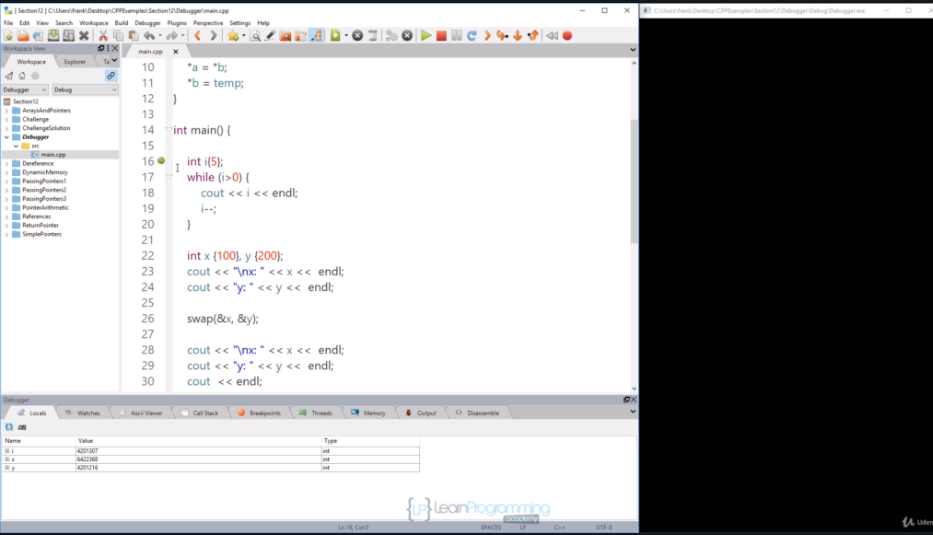
\includegraphics[width=0.4\textwidth]{./Figs/2021-01-15-09-19-44.png}
        % 	\caption{}
        \end{figure}
    
    \item Step in: if the line is a function it allows us execute a break point inside the function.
    \item Step out: if you've pressed step in, steping out will continue where you left off.
    \item Continue/Next: will go to the next line.
    \item Watches: alloc you to check for conditions.
\end{itemize}


%----------------------------------------------------------------------------------------
\section{Section recap}
\begin{itemize}
    \item When to use pointers vs. reference parameters:
        \begin{itemize}
            \item Pass by value.
                \begin{itemize}
                    \item When the function does not modify the actual parameter, and the parameter is small and efficient to copy like simple types (int, char, double, etc.)
                \end{itemize}
            
            \item Pass by reference using a pointer:
                \begin{itemize}
                    \item When the function does moddify the actual parameter, and the parameter is expensive to copy.
                    \item Its OK for a pointer to be null, references cannot be null.
                \end{itemize}
            
            \item Pass by reference usign a pointer to const:
                \begin{itemize}
                    \item Pass by reference using a pointer to \mintinline{cpp}{const}
                        \begin{itemize}
                            \item When the function does not modify the actual parameter, and the parameter is expensive to copy, and its ok for the pointer to be a null value.
                        \end{itemize}
                \end{itemize}
            
            \item Pass by reference using a const pointer to const:
                \begin{itemize}
                    \item When the fucntion does not modify the actual parameter, adn the parameter is expensive to copy, and its OK for the pointer to be a null value, you don't want to modify the pointer itself.
                \end{itemize}
            
            \item Pass by reference using a reference:
                \begin{itemize}
                    \item When the function does modify the actual parameter, and the parameter is expensive to copy, and the parameter will never be a null value.
                \end{itemize}
            
            \item Pass by reference using a const reference:
                \begin{itemize}
                    \item When the function does not modify the actual parameter, and the parameter is expensive to copy, and the parameter will never be a null value.
                \end{itemize}
        \end{itemize}
\end{itemize}
